\documentclass[12pt, letterpaper]{article}

\setcounter{secnumdepth}{3}
%==============Packages & Commands=================
\usepackage{graphicx} % Graphics
\usepackage{indentfirst} % Tells LaTeX to indent every paragraph 
\usepackage{setspace} % To set line spacing
\usepackage{rotating} % For sideways tables/figures
%\usepackage{amsmath} % Some math symbols
\usepackage[margin = .8in]{geometry}
\usepackage{subcaption}
\usepackage{mdwlist}
\usepackage{pifont}
\usepackage{url}
\usepackage{verbatim}
\usepackage{lscape}
\usepackage[hang,flushmargin]{footmisc} 
\usepackage{listings}
\lstset{
  basicstyle=\ttfamily,
  columns=fullflexible,
  frame=single,
  breaklines=true,
  postbreak=\mbox{\textcolor{red}{$\hookrightarrow$}\space},
}
\urlstyle{same}
\usepackage[colorlinks=true,citecolor=blue, breaklinks=true]{hyperref} 
\usepackage[backend=biber,authordate-trad, noibid]{biblatex-chicago}
\usepackage{cleveref} 
\addbibresource{References.bib}
\usepackage{enumitem} %remove space between items.
\usepackage{soul}
\usepackage{float}
\usepackage[export]{adjustbox}
%=========================================
\title{So you want to write your thesis in \LaTeX}
\author{Nguyen Ha\\hatnguyen.267@gmail.com}

%=========================================
\begin{document}
\maketitle
%\doublespacing
\vspace{.3in}

\section{Summary}
We all want a nice-looking thesis. When everyone is roasting your ideas at the defense, at least you can still have the look going for you. Of course, there are many ways to earn this boasting right. Perhaps you're already a wizard in Microsoft Word. Or perhaps you're thinking about \LaTeX, which is a widely used typesetting tool in the academic realm. Although I enjoyed learning this markup language, I also found that I spent a lot of time debugging or just figuring out how certain things work. Assuming that you are unfamiliar with \LaTeX, this document will briefly introduce what it is and why you should (or shouldn't) consider it for your thesis. I'm not an expert in \LaTeX, but I will point you to some useful resources to help you get started. This includes a modified version of the UU thesis template, which should help you produce the department's formatting requirement without much tinkering. 

\section{The pros and cons of \LaTeX}
By this point I hope you haven't made the mistake of looking up \LaTeX in public. Funny name aside, it is a document preparation system, much like your usual Microsoft Word. Unlike in Word, where ``what you see is what you get'', however, you will be producing mostly plain text; the formatting, such as paper size, fonts, and spacing, is defined in a separate section, usually called the ``preamble''. 

Let's be real, \LaTeX is not for every purpose. My friends who study maths and physics will swear by \LaTeX, but in our field, rarely will you ever need to write mathematical equations unless you're working with formal modelling. Other people also praise this tool because it allows you to focus on creating your content, instead of obsessively wrestling with Word's idiosyncracies. I made the choice of writing my thesis in this format after the half-way seminar because I was kind of stubborn, and because I knew it was a widely used tool in academia. I certainly enjoyed the end product--my thesis came together seamlessly without having to worry if I'd missed an indent for a random paragraph--as well as the process of \emph{making things work}. However, if you are new to this typesetting tool, there are certainly some drawbacks. Here, I'll break down what I found to be its pros and cons as a beginner user, and you can decide for yourself.

Pros:
\begin{itemize}[noitemsep]
	\item{It can turn out neat and elegant.}
	\item{It is especially convenient if you plan to conduct statistical analysis in \textsf{R}. The package stargazer, for instance, can produce your tables in \LaTeX format, which renders beautifully.}
	\item{Building the table of content and the list of figures is a breeze. They automatically update every time you compile your files.}
	\item{Referencing, once you've set up everything, is also a breeze. It is also convenient to switch citation style if you want to revise your thesis to submit it elsewhere.}
	\item{It's a useful skill to know if you plan to pursue a career in academia. It is also useful for creating a CV or resume, as there are already hundreds of templates online.}
	\item{In this case, you don't have to start from scratch. Uppsala University has built a template for PhD dissertations, which I have modified to suit the formatting requirements for MA theses at the department.}
\end{itemize}
	
Cons, or common complaints about \LaTeX:

\begin{itemize}[noitemsep]
	\item{Tables are a pain.}
	\item{Diagrams? Thankfully you'll only need one, but, again, this may be time-consuming. See \ref{sssec:num1}.}
	\item{No straight-forward method for word count.}
	\item{It's terrible for collaboration. Your supervisor and classmates will have to edit your drafts as PDF files, and we all know how annoying that can be.} 
	\item{UU doesn't provide any technical support for \LaTeX, and not all your classmates will be on the same boat. In other words, you will be swimming on your own.}
	\item{Many people will tell you that \LaTeX is better for productivity, but this may not be true. There has been many Internet wars, even \href{https://journals.plos.org/plosone/article?id=10.1371/journal.pone.0115069}{an experiment}, on the topic with no clear consensus reached. Overall, \LaTeX may have a steeper learning curve and, therefore, require more time and effort.} 
\end{itemize}
	
At the end of the day, it all boils down to your personal preference and how much time you have on hand. Most things you can do with \LaTeX can be achieved with Microsoft Word. For example, building a table of content in Word is just as easy using the built-in Outline mode. On the other hand, most of the cons can be addressed, which I have done in the sections to follow. In short, if the deadline is looming on the horizon, stick with whatever tool that you already know best. For the rest of the document, let's pretend that you are somewhat interested in learning this skill.

\section{Getting started}
\subsection{The setup}
To begin, you need a \TeX editor and compiler. There are many options on the market--many of which are free, and often the choice depends largely on your operating system. At the very minimum, you can write your document in Notepad and compile it in a command terminal. However, I'd recommend going for a \LaTeX-specific editor. As a Windows user, I have only tried the classic combination of TeXworks/MiKTeX and very much liked the simplicity. TeXstudio is also a popular free editor, and it provides shortcuts for common \LaTeX syntaxes, e.g. how to write letters with accent, attach graphics, and even convert outputs into Word documents. Other paid options include extra tools that make your life easier. The free version of Overleaf, for example, is online and allows you to preview your PDF as you go. The paid version also supports collaboration between authors. Here is a list of TeX clients so you can shop around and find out which one you like best.\\
TeXworks/MiKTeX: \href{http://www.tug.org/texworks/}{http://www.tug.org/texworks/}\\
TeXstudio: \href{https://www.texstudio.org/}{https://www.texstudio.org/}\\
Overleaf: \href{https://www.overleaf.com/}{https://www.overleaf.com/}

\subsection{Organizing your files}
The first thing you should start with is organizing your thesis draft folder. During the compilation process, \LaTeX will produce many temporary files. If you're putting your main thesis file in a big folder, for instance, it will make that folder look like trash. 

Let's start in your main working directory. This is where your main .tex file and the template file should do. Then, following the advice of Mori \autocite*{mori2007writing}, I created three folders: \verb|\bib| for the bibliography file, \verb|\fig| for figures, and \verb|\tex| for all the chapters. This means that you write each chapter separately, which will then be called on in your main \verb|.tex| file and compiled. There is no preamble in the chapter file, as all formatting choices are configured in the main \verb|.tex| file, as well as in the \verb|.cls| template.

\subsection{Co-opting the UU Thesis Template}
Uppsala University has constructed its own \LaTeX template for PhD dissertations, which can be downloaded \href{https://libguides.ub.uu.se/Thesis/Template_LaTeX}{here}. Unfortunately, their website says that there is no longer any official support for \LaTeX. Furthermore, the template requires some tweaking, because it is originally designed with a \emph{printed} dissertation in mind. This means that you will find blank pages which are there so that a chapter could begin on a right-sided page of a book, but which you don't really need in your Master's thesis. But, the template can still be useful, especially if you are just starting out with \LaTeX and do not want to spend too much time figuring out the smaller details, such as font sizes for each heading level or page margins. 

In this folder, you will find two documents titled \verb|Overall.tex| and \verb|UU_Thesis_Template.cls|. \verb|Overall.tex| will be your main working document, on which you will run the compilation process to obtain the final \verb|.pdf| product. In the preamble section of this file, I have added all the useful packages that you may need. I have also adjusted the \verb|UU_Thesis_Template.cls| file so that it will help you meet the formatting requirements for the MA thesis at the department.

\subsubsection{Cover page}
To add information to the cover page, search for the phrase ``cover page'' in the template file.

\subsubsection{Tables}
For descriptive and result tables, the packages \verb|stargazer| and \verb|texreg| in \textsf{R} can both produce \LaTeX outputs, which you can effortlessly copy and paste into your document. The problem begins when you have tables that are longer than one page, or tables containing paragraphs. In these cases, consider the merits of the packages \verb|tabular*|, \verb|tabularx|, \verb|tabulary|, and \verb|longtable|. 

\subsubsection{Attaching graphics and diagrams} \label{sssec:num1}
For diagrams, \verb|tikz| is common choice, but it is by no means the best choice. If you like coordinate geometry, perfect. If not, just create your diagram with your favorite graphic tool (Kristine recommended \href{https://www.draw.io/}{https://www.draw.io/}), and insert it as a graphic using the package \verb|graphicx|.

\subsubsection{Bibliography}
As mentioned above, creating a bibliography in \LaTeX is a breeze. I recommend using \verb|biblatex| and any reference management software of your choice (I use the free Zotero). In the preamble of the \verb|Overall.tex| file, you will find that the document is set to produce the Chicago author-date citation format. All you need to do is to produce a \verb|.bib| file from your reference manager, put it in the appropriate folder, and call on it in the \verb|\addbibresource{}| tag. After that, run the compilation process in the following order: \verb|pdflatex -> Biber -> pdflatex x2|. 

Here is a cheat sheet for \verb|biblatex|: \\
\href{http://tug.ctan.org/info/biblatex-cheatsheet/biblatex-cheatsheet.pdf}{\nolinkurl{http://tug.ctan.org/info/biblatex-cheatsheet/biblatex-cheatsheet.pdf}}

\subsubsection{Word count}
There is no straightforward tool to calculate word count for LaTeX. The most popular and accessible option is TeXcount: \href{https://app.uio.no/ifi/texcount/index.html}{https://app.uio.no/ifi/texcount/index.html}. Or, convert your document to Word format (see section \ref{sssec:num2}).

\subsubsection{Quotes at the start of your chapter}
There are several approaches to this. Here is one example from my own thesis. If you define the following command in your preamble...

\begin{lstlisting}
\newcommand{\chapquote}[3]{\begin{quotation} \textit{#1} \end{quotation} \begin{flushright} - #2, \textit{#3}\end{flushright} }
\end{lstlisting}

and add this at the beginning of your chapter... 

\begin{lstlisting}
\chapter{Introduction}
\chapquote{``All wars are fought twice, the first time on the battlefield, the second time in memory".}{Viet Thanh Nguyen}{Nothing Ever Dies}
\end{lstlisting}
... you will get something similar to Figure \ref{fig1}.

\begin{figure}
\centering
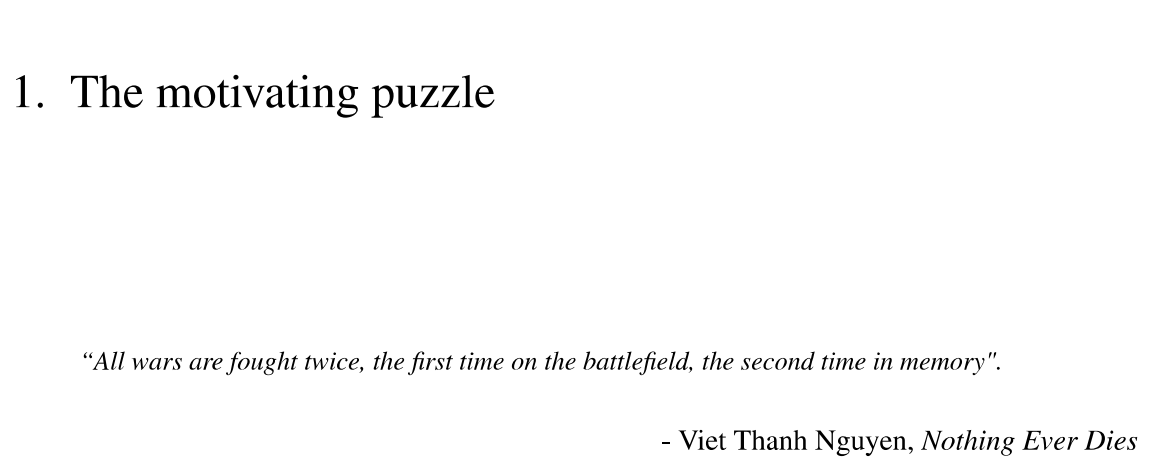
\includegraphics[width=\linewidth, frame]{introquote.png}
\caption{An example of quote.}
\label{fig1}
\end{figure}

You may also find other suggestions on Stack Exchange. As this example shows, defining a new command in the preamble is one way to add customized formatting to your documents. The UU Thesis Template is chockfull of its own commands, for instance. So if you are feeling adventurous, and you have not found an acceptable solution on Stack Exchange for what you have in mind, this is how you could go about owning this \LaTeX beast.

\subsubsection{Converting between formats} \label{sssec:num2}
A common complaint about \LaTeX is that it does not faciliate collaboration among authors. Your end-product is almost always a \verb|.pdf| file, which makes it difficult to comment on or highlight typographies. But, this is no longer a problem with Pandoc -- a document converter that works with almost all markup formats. See their homepage for details and instructions for download: \href{https://pandoc.org/index.html}{https://pandoc.org/index.html}. 

For a concise guideline on how to convert a \verb|.tex| file into \verb|.docx|, see this link: \href{https://medium.com/@zhelinchen91/how-to-convert-from-latex-to-ms-word-with-pandoc-f2045a762293}{\nolinkurl{https://medium.com/@zhelinchen91/how-to-convert-from-latex-to-ms-word-with-pandoc-f2045a762293}}.

As an example, I have carried out the same process on this document and attached the \verb|.docx| output in this folder. 

\section{Final thoughts}
Writing with \LaTeX may be annoying at the start, but things will get smoother once you have everything set up, and the end result can be rewarding. I hope that this document has been useful in giving you an overall picture of this markup tool. If you spot any bug with the template, or have any suggestion to make it better, please let me know. 

Here are some additional resources:
\begin{itemize}[noitemsep]
\item{Stack Exchange: \href{https://tex.stackexchange.com/}{https://tex.stackexchange.com/}}
\item{An introductory guideline to writing your thesis in \LaTeX by \textcite{mori2007writing}.}
\end{itemize}

Best of luck with your thesis!
 
 


\printbibliography



\end{document}